\section{Data selection}
\lb{sec:data}

\begin{figure*}[h]
	\makebox[\textwidth][c]{
    	\begin{subfigure}{0.3\textwidth}
        	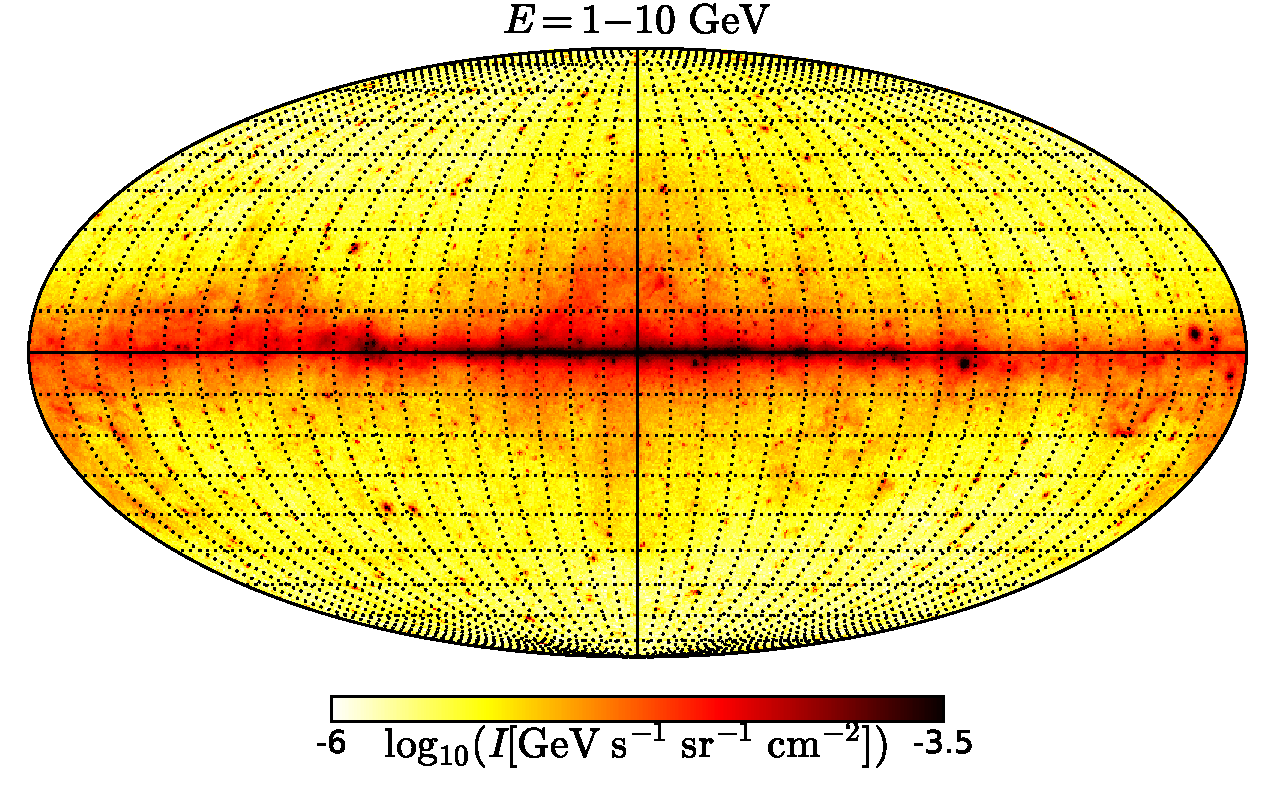
\includegraphics[width=\textwidth]{plots/Mollweide_data_source_range_0.pdf}
    	\end{subfigure} 
    	\begin{subfigure}{0.3\textwidth}
        	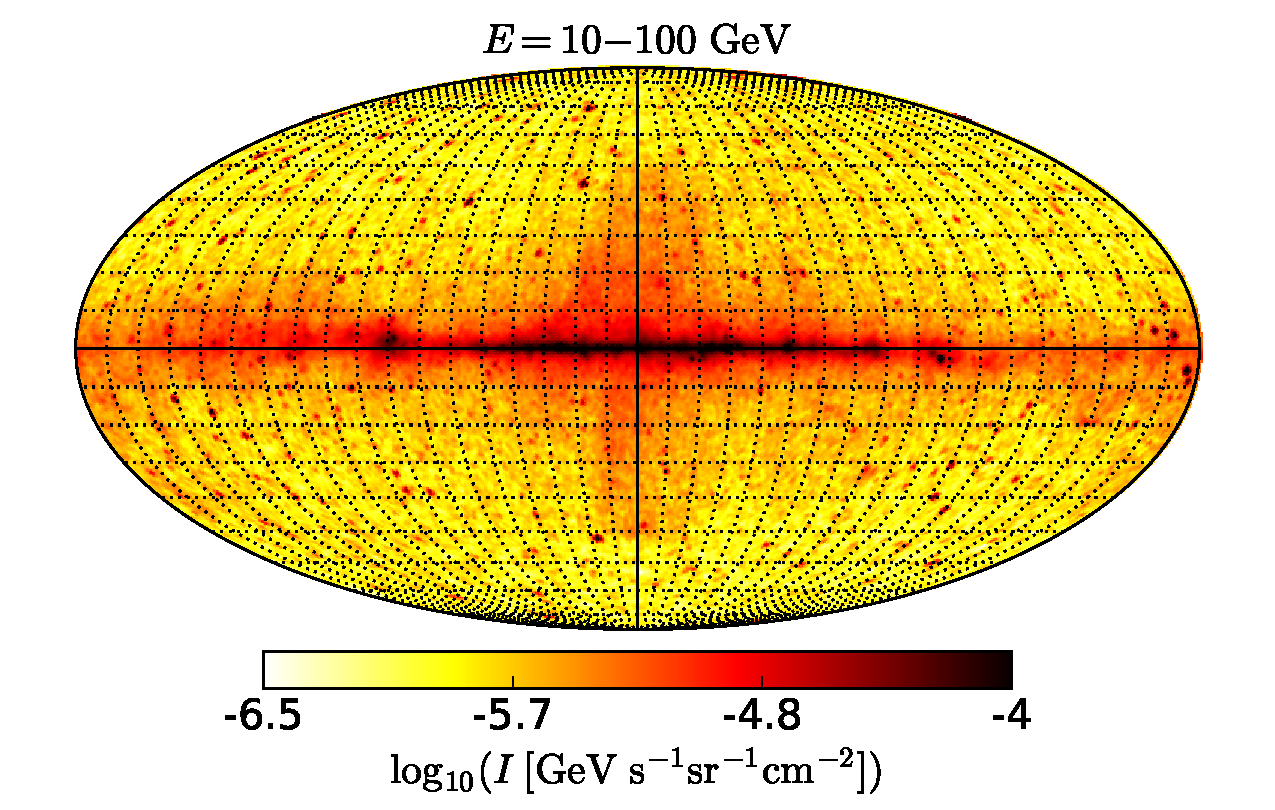
\includegraphics[width=\textwidth]{plots/Mollweide_data_source_range_1.pdf}
    	\end{subfigure}
    	\begin{subfigure}{0.3\textwidth}
        	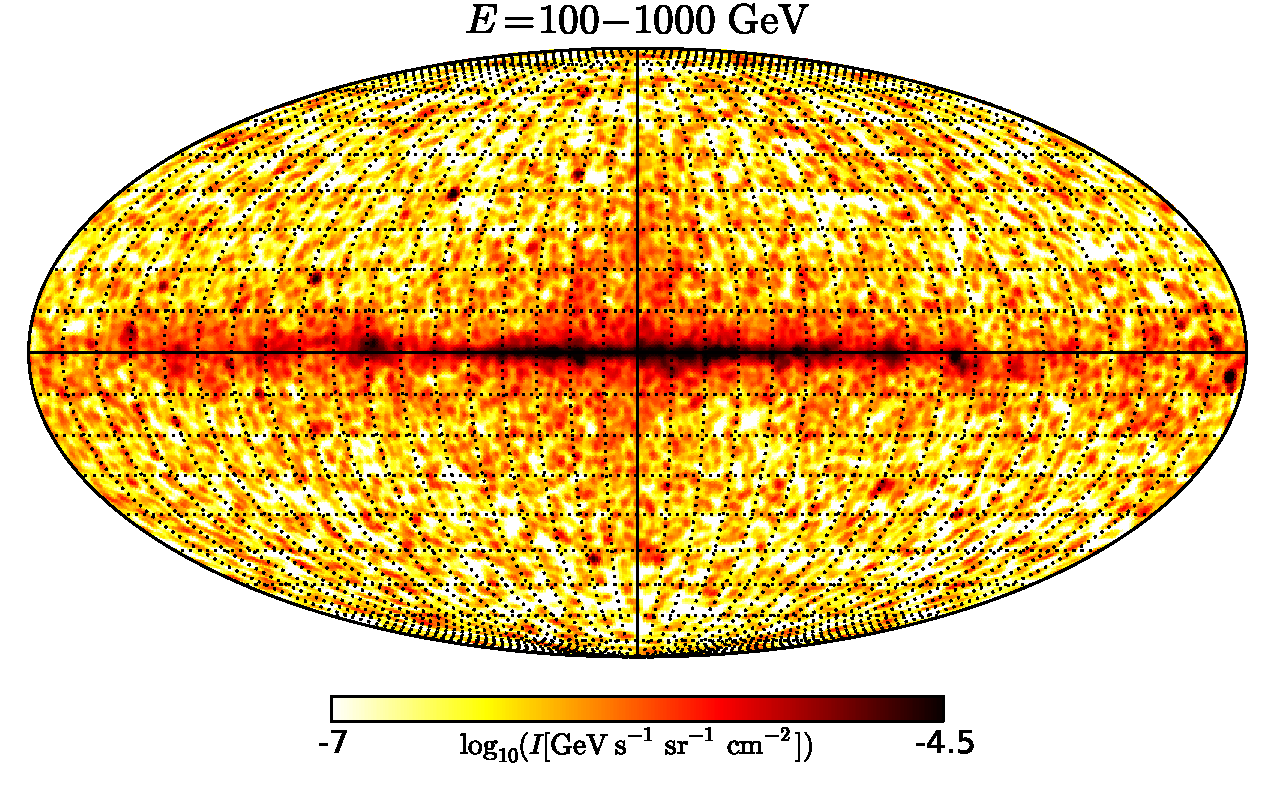
\includegraphics[width=\textwidth]{plots/Mollweide_data_source_range_2.pdf}
    	\end{subfigure}
    }
  	\caption{9-year \Fermi data in three different energy ranges.}
  	\label{fig:Maps_data}
\end{figure*}

The main goal of the analysis is a study of a relatively small region $\lesssim 10^\circ$ from the GC for energies $\gtrsim 1$ GeV.
We use 9 years of the \Fermi-LAT Pass 8 Source class events
between August 4, 2008  and August 3, 2017 ({\Fermi} Mission Elapsed Time 239557418\,s -- 523411376\,s)
with energies between 316 MeV $ = 10^{2.5}$ MeV
and 1 TeV separated in 21 logarithmic energy bins (6 bins per decade).
The selection of the events is performed with the standard quality cuts.
In order to avoid contamination from gamma rays produced in interactions of cosmic ray in the Earth atmosphere, 
we select events with the zenith angles $\theta < 100^{\circ}$,
which is sufficient for energies above 316 MeV.
We calculate the exposure and PSF using the {\Fermi}-LAT Science Tools package version 
10-01-01 available from the {\Fermi} Science Support Center\footnote{\url{http://fermi.gsfc.nasa.gov/ssc/data/analysis/}} 
with the P8R2\_SOURCE\_V6 instrument response functions.
For spatial binning we use HEALPix\footnote{\url{http://sourceforge.net/projects/healpix/}} \citep{2005ApJ...622..759G} scheme with a pixelization of order 7  ($\approx 0\degr\!\!.46$ pixel size). 
